%%%%%%%%%%%%%%%%%%%%%%%%%%%%%%%%%%%%%%%%%
% Beamer Presentation
% LaTeX Template
% Version 1.0 (10/11/12)
%
% This template has been downloaded from:
% http://www.LaTeXTemplates.com
%
% License:
% CC BY-NC-SA 3.0 (http://creativecommons.org/licenses/by-nc-sa/3.0/)
%
%%%%%%%%%%%%%%%%%%%%%%%%%%%%%%%%%%%%%%%%%

%----------------------------------------------------------------------------------------
%	PACKAGES AND THEMES
%----------------------------------------------------------------------------------------

\documentclass{beamer}

\mode<presentation> {

% The Beamer class comes with a number of default slide themes
% which change the colors and layouts of slides. Below this is a list
% of all the themes, uncomment each in turn to see what they look like.

%\usetheme{default}
%\usetheme{AnnArbor}
%\usetheme{Antibes}
%\usetheme{Bergen}
%\usetheme{Berkeley}
%\usetheme{Berlin}
%\usetheme{Boadilla}
%\usetheme{CambridgeUS}
%\usetheme{Copenhagen}
%\usetheme{Darmstadt}
%\usetheme{Dresden}
\usetheme{Frankfurt}
%\usetheme{Goettingen}
%\usetheme{Hannover}
%\usetheme{Ilmenau}
%\usetheme{JuanLesPins}
%\usetheme{Luebeck}
%\usetheme{Madrid}
%\usetheme{Malmoe}
%\usetheme{Marburg}
%\usetheme{Montpellier}
%\usetheme{PaloAlto}
%\usetheme{Pittsburgh}
%\usetheme{Rochester}
%\usetheme{Singapore}
%\usetheme{Szeged}
%\usetheme{Warsaw}

% As well as themes, the Beamer class has a number of color themes
% for any slide theme. Uncomment each of these in turn to see how it
% changes the colors of your current slide theme.

%\usecolortheme{albatross}
%\usecolortheme{beaver}
%\usecolortheme{beetle}
%\usecolortheme{crane}
%\usecolortheme{dolphin}
%\usecolortheme{dove}
%\usecolortheme{fly}
%\usecolortheme{lily}
%\usecolortheme{orchid}
%\usecolortheme{rose}
%\usecolortheme{seagull}
%\usecolortheme{seahorse}
%\usecolortheme{whale}
%\usecolortheme{wolverine}

%\setbeamertemplate{footline} % To remove the footer line in all slides uncomment this line
%\setbeamertemplate{footline}[page number] % To replace the footer line in all slides with a simple slide count uncomment this line

%\setbeamertemplate{navigation symbols}{} % To remove the navigation symbols from the bottom of all slides uncomment this line
}

\usepackage{graphicx} % Allows including images
\usepackage{booktabs} % Allows the use of \toprule, \midrule and \bottomrule in tables
\usepackage{color}


%\newtheorem{theorem}{Theorem}
\newtheorem{protocol}{Protocol}
%\newtheorem{lemma}{Lemma}
\newtheorem{claim}{Claim}
\newtheorem{property}{Property}



\newcommand{\bbZ}{\mathbb{Z}}
\newcommand{\calC}{\mathcal{C}}
\newcommand{\calI}{\mathcal{I}}
\newcommand{\calM}{\mathcal{M}}
\newcommand{\calK}{\mathcal{K}}
\newcommand{\opt}{\text{OPT}}
\newcommand{\knowopt}{{\sc KnowOpt}}
\newcommand{\alg}{\text{ALG}}

\newcommand{\emRed}[1][]{\textcolor{blue} #1}
\newcommand{\bbR}{\mathbb{R}}

\DeclareMathOperator*{\argmin}{arg\,min}
\DeclareMathOperator*{\argmax}{arg\,max}

%----------------------------------------------------------------------------------------
%	TITLE PAGE
%----------------------------------------------------------------------------------------

\title[Submodular Maximization]{Submodular Maximization\\\small{advances in distributed/streaming computing}} % The short title appears at the bottom of every slide, the full title is only on the title page

\author{Jiecao Chen} % Your name
\institute[IUB] % Your institution as it will appear on the bottom of every slide, may be shorthand to save space
{
Indiana University Bloomington \\ % Your institution for the title page
\medskip
\textit{jiecchen@indiana} % Your email address
}
\date{\today} % Date, can be changed to a custom date

\begin{document}

\begin{frame}
\titlepage % Print the title page as the first slide
\end{frame}

\begin{frame}
\frametitle{Overview} % Table of contents slide, comment this block out to remove it
\tableofcontents % Throughout your presentation, if you choose to use \section{} and \subsection{} commands, these will automatically be printed on this slide as an overview of your presentation
\end{frame}

%----------------------------------------------------------------------------------------
%	PRESENTATION SLIDES
%----------------------------------------------------------------------------------------

%------------------------------------------------
\section{Introduction to Submodularity} % Sections can be created in order to organize your presentation into discrete blocks, all sections and subsections are automatically printed in the table of contents as an overview of the talk
%------------------------------------------------

\subsection{Definitions} % A subsection can be created just before a set of slides with a common theme to further break down your presentation into chunks

\begin{frame}
\frametitle{Definitions of Submodularity}
\begin{definition}[submodular concave]
  \label{def:sub-concave}
  A function $f:~2^V \rightarrow \bbR$ is \emRed{submodular} if for any $A, B \subseteq V$, we have that:
  \begin{equation}
    \label{eq:sub-concave}
    f(A) + f(B) \geq f(A \cup B) + f(A \cap B).
  \end{equation}
\end{definition}

An alternate equivalent definition is more interpretable in many situations.

\begin{definition}[diminishing returns]
  \label{def:sub-diminishing}
  A function $f: 2^V \rightarrow \bbR$ is \emRed{submodular} if for any $A \subseteq B \subset V$, and $v \in V\backslash B$, we have that:
  \begin{equation}
    \label{eq:sub-diminishing}
    f(A + v) - f(A) \geq f(B + v) - f(B).
  \end{equation}
\end{definition}

\end{frame}

%------------------------------------------------

\begin{frame}
\frametitle{Modular Functions}
\begin{definition}[Modularity]
  \label{def:modular}
  A function $f: 2^V \rightarrow \bbR$ is \emRed{modular} if for any $A \subseteq B \subset V$, and $v \in V\backslash B$, we have that:
  \begin{equation}
    \label{eq:modular}
    f(A + v) - f(A) = f(B + v) - f(B).
  \end{equation}
\end{definition}
Notably, a modular function $f$ can always be written as
$$f(S) = f(\emptyset) + \sum_{v\in S} \left( f(\{v\}) - f(\emptyset) \right)$$
for any $S \subseteq V$. If we further assume $f(\emptyset) = 0$ (in this case, we call $f$ \emRed{normalized} or \emRed{proper}), we have a simplified expression,

$$f(S) = \sum_{v\in S} f(\{v\}).$$

\end{frame}

\begin{frame}
\frametitle{Monotonitcity}
\begin{definition}[Monotonitcity]
  A set function $f: 2^V \rightarrow  \bbR$ is said to be non-decreasing if for any $A\subseteq B \subseteq V$, $f(A) \leq f(B)$. Non-increasing set functions are defined in the similar way.
\end{definition}
When we say a submodular function is monotone, we mean it is non-decreasing.
\end{frame}


\subsection{Properties}
\begin{frame}
\frametitle{Properties}

Submodularity is closed under addition.
\begin{property}
  \label{prop:addition}
  Let $f_1, f_2: 2^V \rightarrow \bbR$ be two submodular functions. Then 
  $$f: 2^V\rightarrow \bbR~~\text{with}~~ f(A) = \alpha f_1(A) + \beta f_2(A)$$ 
is submodular for any fixed $\alpha, \beta \in \bbR^+$.
\end{property}

Submodularity is preserved under restriction.
\begin{property}
  \label{prop:restriction}
  Let $f: 2^V \rightarrow \bbR$ be a submodular function. Let $S\subseteq V$ be a fixed set. Then
$$f':2^V \rightarrow \bbR~~\text{with}~~f'(A) = f(A\cap S)$$
is submodular.
\end{property}
\end{frame}


\begin{frame}
\frametitle{Properties cont.}
The following property can be useful when we show that the negative of the objective function of k-median problem is submodular.
\begin{property}
  \label{prop:max}
Consider $V$ as a set of indices. Let $\mathbf{c}\in \bbR^V$ be a fixed vector, $c_i$ its $i$th coordinate. Then 
$$f:2^V \rightarrow \bbR~~\text{with}~~ f(A) = \max_{j\in A}c_i$$ 
is submodular.
\end{property}
\end{frame}



\subsection{Constraints}
\begin{frame}
\frametitle{Constraints}
\begin{block}{Submodular Maximization Problem}
A submodular maximization problem usually has the following form:

\begin{equation}
  \label{eq:optimization}
  \argmax_{I\in\calI} f(I),
\end{equation}
\end{block}
where $f$ is a submodular function and $\calI \subseteq 2^V$ is the collection of all feasible solutions. We call $\calI$ the \emRed{constraint} of the optimization problem.
\end{frame}


\begin{frame}
\frametitle{Constraints}

\begin{block}{$\calI$ is important!}
The structure of $\calI$ plays a crucial role in submodular optimization:
\begin{itemize}
\item Different constraints have different hardness results.
\item Normally the difficulty increases when the constraint becomes more general.
\end{itemize}
\end{block}

\begin{block}{Popular constraints}
Some popular constraints:
\begin{itemize}
\item Cardinality constraint
\item Knapsack constraint
\item Matroid constraint
\item Matching
\item $p$-System
\item ...
\end{itemize}
\end{block}
\end{frame}



\begin{frame}
\frametitle{Constraints cont.}
First we define hereditary set systems.
\begin{definition}[Hereditary]
  \label{def:hereditary}
  A constraint $\calI \subseteq 2^V$ is said to be \emRed{hereditary} if 
$$I\in\calI \implies J\in\calI ~\text{for any}~J\subseteq I.$$
A hereditary constraint is sometimes called an \emRed{independent system} and each $I\in\calI$ is called an \emRed{independent set}. 
\end{definition}
\textbf{All constraints we will discuss are hereditary.}
\end{frame}

\begin{frame}
  \frametitle{Constraints cont.}
  \begin{block}{Cardinality}
    \emRed{Cardinality constraint}: $\calI = \{A \subseteq V ~|~ |A| \leq k\}$
  \end{block}

  \begin{block}{Knapsack}
   \emRed{Knapsack Constraint}: each $i \in V$ is assigned a weight $w_i \geq 0$,  $\calI = \{S \subseteq V ~|~ \sum_{i\in S} w_i \leq W \}$.
  \end{block}


  \begin{block}{Matching}
     \emRed{Matching}: given a graph $G = (V, E)$, a \emph{Matching} is a set $S\subseteq E$ such that no edges in $S$ share common vertex.
  \end{block}

  \begin{block}{Matroid}
    \emRed{Matroid} is the generalization of the independence concept in linear algebra;
    omit details here ...
  \end{block}


\end{frame}




\begin{frame}
  \frametitle{$p$-System}
\emRed{$p$-system} is the most general constraint we will discuss in this survey, it includes graph matching, $p$-matchoid (therefore matroid) and many others as special cases.

\begin{block}{Definition of $p$-System}
Let $(V, \calI)$ be a set system and $\calI$ hereditary.  Let $\mathcal{B}(A)$ be the collection of all bases of $A$.

$$\calI = \{ A \subset V ~|~ \frac{\max_{S\in\mathcal{B}(A)}|S|}{\min_{S\in\mathcal{B}(A)}|S|} \leq p \}.$$
\end{block}

\textbf{Note:} a \emRed{base} of $A$ is the maximal independent set included in $A$. 

\end{frame}


\begin{frame}
  \frametitle{Hierarchy of constraints}
  \begin{figure}[!ht]
    \centering
    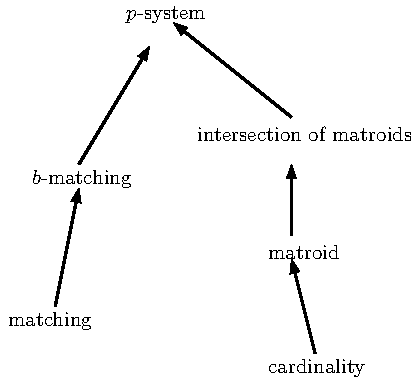
\includegraphics[width=0.7\textwidth]{figures/hh}
  \end{figure}
\end{frame}


\begin{frame}
  \frametitle{Hierarchy of constraints (extended)}
  \begin{figure}[!ht]
    \centering
    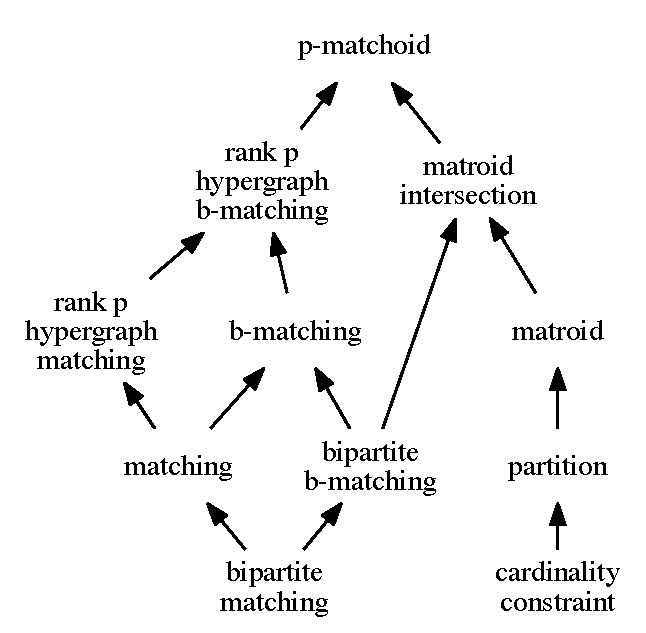
\includegraphics[width=0.7\textwidth]{figures/hierarchy}
  \end{figure}
\end{frame}


%------------------------------------------------



\begin{frame}
\frametitle{Multiple Columns}
\begin{columns}[c] % The "c" option specifies centered vertical alignment while the "t" option is used for top vertical alignment

\column{.45\textwidth} % Left column and width
\textbf{Heading}
\begin{enumerate}
\item Statement
\item Explanation
\item Example
\end{enumerate}

\column{.5\textwidth} % Right column and width
Lorem ipsum dolor sit amet, consectetur adipiscing elit. Integer lectus nisl, ultricies in feugiat rutrum, porttitor sit amet augue. Aliquam ut tortor mauris. Sed volutpat ante purus, quis accumsan dolor.

\end{columns}
\end{frame}

%------------------------------------------------
\section{Applications}
%------------------------------------------------

\begin{frame}
\frametitle{Table}
\begin{table}
\begin{tabular}{l l l}
\toprule
\textbf{Treatments} & \textbf{Response 1} & \textbf{Response 2}\\
\midrule
Treatment 1 & 0.0003262 & 0.562 \\
Treatment 2 & 0.0015681 & 0.910 \\
Treatment 3 & 0.0009271 & 0.296 \\
\bottomrule
\end{tabular}
\caption{Table caption}
\end{table}
\end{frame}

%------------------------------------------------

\begin{frame}
\frametitle{Theorem}
\begin{theorem}[Mass--energy equivalence]
  $E = mc^2$
\end{theorem}
\end{frame}

%------------------------------------------------


% \begin{frame}[fragile] % Need to use the fragile option when verbatim is used in the slide
% \frametitle{Verbatim}
% \begin{example}[Theorem Slide Code]
% \begin{verbatim}
% \begin{frame}
% \frametitle{Theorem}
% \begin{theorem}[Mass--energy equivalence]
% $E = mc^2$
% \end{theorem}
% \end{frame}
% \end{verbatim}
% \end{example}
% \end{frame}

%------------------------------------------------

\begin{frame}
\frametitle{Figure}
Uncomment the code on this slide to include your own image from the same directory as the template .TeX file.
%\begin{figure}
%\includegraphics[width=0.8\linewidth]{test}
%\end{figure}
\end{frame}

%------------------------------------------------

\begin{frame}[fragile] % Need to use the fragile option when verbatim is used in the slide
\frametitle{Citation}
An example of the \verb|\cite| command to cite within the presentation:\\~

This statement requires citation \cite{p1}.
\end{frame}

%------------------------------------------------
%------------------------------------------------
\section{Streaming Submodular Maximization}
%------------------------------------------------


\begin{frame}
\frametitle{References}
\footnotesize{
\begin{thebibliography}{99} % Beamer does not support BibTeX so references must be inserted manually as below
\bibitem[Smith, 2012]{p1} John Smith (2012)
\newblock Title of the publication
\newblock \emph{Journal Name} 12(3), 45 -- 678.
\end{thebibliography}
}
\end{frame}

%------------------------------------------------

%------------------------------------------------
\section{Distributed Submodular Maximization}
%------------------------------------------------


\begin{frame}
\Huge{\centerline{The End}}
\end{frame}

%----------------------------------------------------------------------------------------



\bibliographystyle{abbrv}
\bibliography{survey.bib}

\end{document} 